% Comparisons
% Gelu (baseline) with Adaptive gelu
% ReLU with PReLU (Adaptive reslu)
% SiLU with Swish
% ReLU with GeLu

\begin{figure*}[ht]
    \centering
    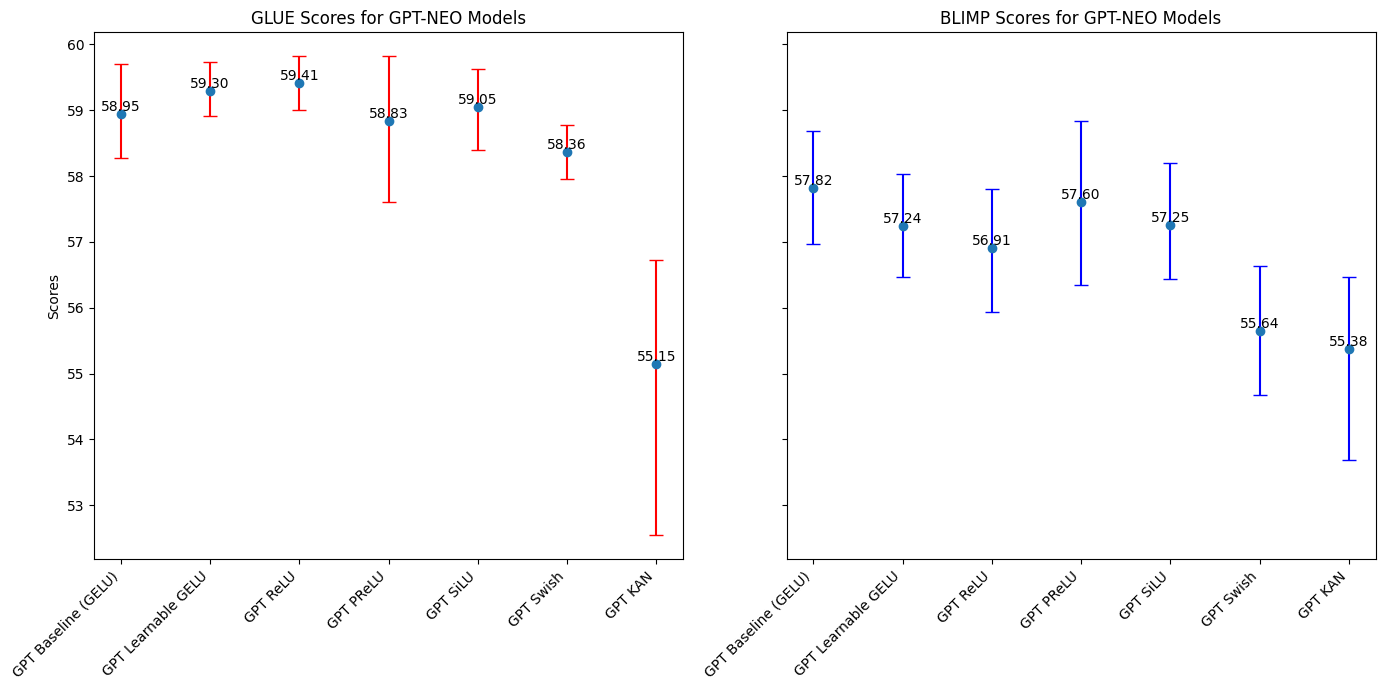
\includegraphics[width=\columnwidth * 2]{figures/gpt-intervals.png}
    \caption{GLUE and BLiMP scores for GPT NEO models with 95\% confidence intervals}
    \label{fig:gpt-intervals}
\end{figure*}

\begin{figure*}[h]
    \centering
    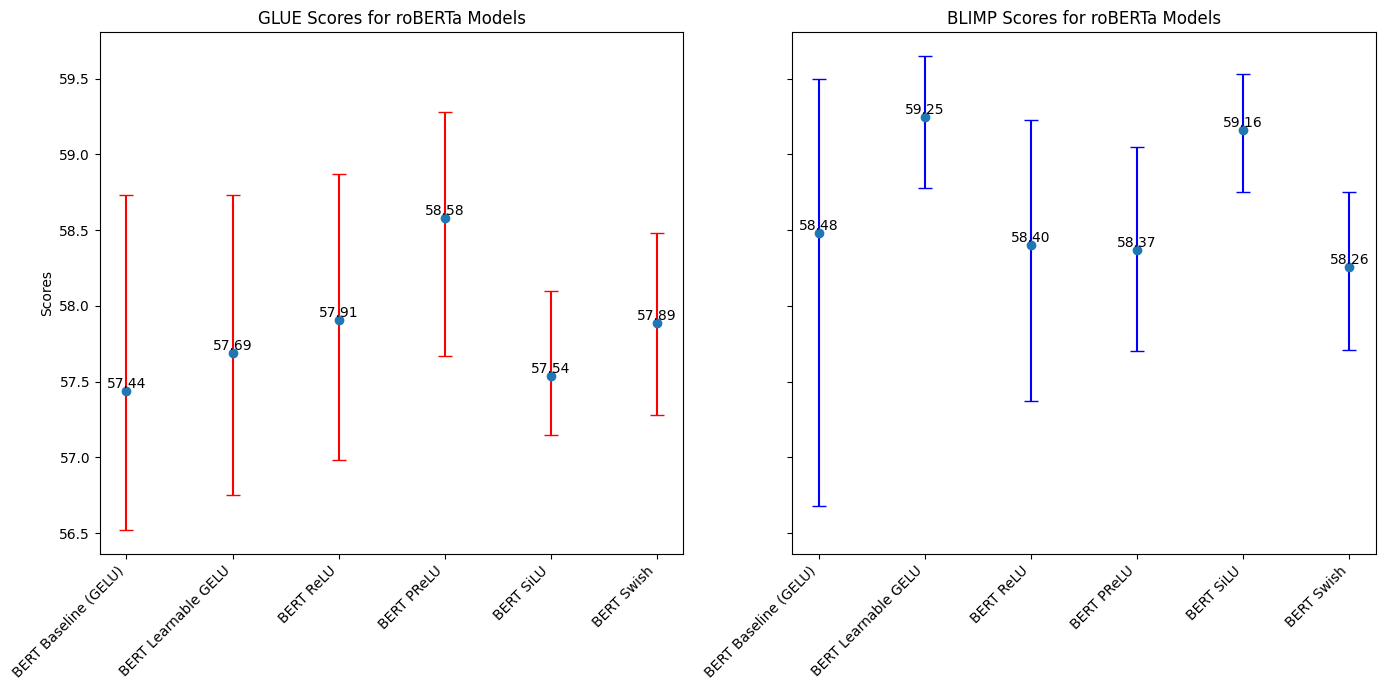
\includegraphics[width=\columnwidth * 2]{figures/roberta-intervals.png}
    \caption{GLUE and BLiMP scores for roBERTa models with 95\% confidence intervals}
    \label{fig:roberta-intervals}
\end{figure*}

\section{Results} % PAST TENSE!!!
\label{sec:results}
The evaluation results for the BLiMP and GLUE datasets are displayed in Figures \ref{fig:gpt-intervals} and \ref{fig:roberta-intervals}. We calculated the mean scores and 95\% confidence intervals for BLiMP and GLUE after performing bootstrap resampling for 10,000 samples.

For the first research question, which compares the baseline GELU activation function with its predecessor RELU, the results are inconclusive. The differences in scores between the two activation functions are statistically insignificant. With the GLUE means even being higher for both roBERTa and NEO models are marginally higher with the RELU activation function, the confidence intervals overlap, indicating no significant difference.

Regarding the second research question, which compares static activation functions with their adaptive counterparts, the findings are similarly inconclusive. The differences between static and adaptive activation functions are minor, and the overlapping confidence intervals suggest no statistical significance.

For the third research question, which was only evaluated on the GPT-NEO model due to time constraints, the results show a statistically significant difference. The KAN model performed worse than all other models on GLUE and worse than most models on BLiMP.

Training times across all models were consistent when using the same GPU. On the A100 GPU, training times were approximately 1 hour and 40 minutes, while on the V100 GPU, training times were around 2 hours and 20 minutes. Not all experiments were conducted on the A100 GPU due to time constraints and DelftBue \cite{DHPC2024} availability. The KAN network models were outliers, with training times averaging around 3 hours and 30 minutes on the A100 GPU and 4 hours and 50 minutes on the V100 GPU, which was expected. More details on the training times can be found in Table \ref{tab:average-times} and Table \ref{tab:all-results}.